\subsection[定义和性质]{复变函数的积分}
有了复变函数微分的基础,我们现在来讨论积分.复变函数的积分的定义可以同实变函数积分的类比得到.
在复平面上取一个路径$\ell$,起终点为$A(z_0),B(z_n)$,沿着该路径定义了一连续函数$f(z)$,用$n-1$个点$z_1, z_2,\cdot, z_{n-1}$将该路径
$\ell$分成$n$个线段(见图\ref{fig:complex_integral}).函数$f(z)$在线段$z_{k-1}\rightarrow z_{k}$上任意一点$\xi_k$的值乘上线段的长度$\Delta z_k = z_k - z_{k-1}$并求和,即
\begin{equation}
    S_n = \sum_{k=1}^{n} f(\xi_k) (z_{k} - z_{k-1}) .
\end{equation}
\begin{figure}[htbp]
    \centering
    \chapter{定积分的计算}
对于实变函数的定积分,我们已经学会了一些积分技巧,如变量代换,分部积分等.这一章我们将介绍利用留数定理的积分技巧,并介绍以物理学家Richard P. Feynman命名的
特殊技巧.

% \section{留数定理应用}
\subsection{三角函数的积分}
考虑积分区间为$\left[ 0, 2\pi \right]$,被积函数为三角函数有理式的积分
\begin{equation}
    \int_{0}^{2\pi} R(\cos{x}, \sin{x}) dx,
\end{equation}
当实变数 $x$ 从 0 变到 $2 \pi$ 时, 复变数 $z=e^{\imath x}$ 从 $z=1$ 出发沿单位圆 $|z|=1$ 逆时针 走一圈又回到 $z=1$,
实变定积分化为复变回路积分, 就可以应用留数定理了. 至于实变定积分里的 $\cos x, \sin x$ 和 $d x$, 作如下变换:
$$
\cos x=\frac{1}{2}\left(z+z^{-1}\right), \quad \sin x=\frac{1}{2 \imath}\left(z-z^{-1}\right), \quad d x=\frac{1}{\imath z} d z .
$$
于是, 原积分化为
$$
I=\oint_{|z|=1} R\left(\frac{z+z^{-1}}{2}, \frac{z-z^{-1}}{2 \imath}\right) \frac{d z}{\imath z}
$$
利用留数定理即可求得.

\begin{example}
求定积分\[I=\int_0^{2 \pi} \frac{d \theta}{1+a \cos \theta}, \quad|a|<1 \]
\end{example}
\begin{solution}
    根据上面的方法,可得
    \[
        \begin{aligned}
        I & =-\imath \oint_{|z|=1} \frac{d z}{z\left[1+(a / 2)\left(z+z^{-1}\right)\right]} \\
        & =-\imath \frac{2}{a} \oint \frac{d z}{z^2+(2 / a) z+1} .
        \end{aligned}
    \]
    两个极点分别为
    \[
        z_1=-\frac{1+\sqrt{1-a^2}}{a} \quad \text {和} \quad z_2=-\frac{1-\sqrt{1-a^2}}{a}
    \]
    不难看出,$z_1$在单位圆外,$z_2$在单位圆内.积分可以写成
    \[
      \oint \frac{dz}{(z-z_1)(z-z_2)}   
    \]
    留数则为$\frac{1}{z_2 - z_1}$, 利用留数定理可得 
    \[
      I=  -\imath \frac{2}{a} 2\pi\imath \frac{1}{z_2 - z_1} = \frac{2}{\sqrt{1 - a^2}} . 
    \]
\end{solution}



\subsection{积分上下限为$( -\infty, \infty)$}
 考虑如下形式的定积分
 \[
    \int_{-\infty}^{\infty} f(x) dx
 \]
 我们先讨论复变函数 $f(z)$ 在实轴上没有奇点的情况,有奇点的情况后面讨论. 
被积函数在上半平面除有限个奇点外是解析的; 当 $z$ 在上半平面及实轴上 $\to \infty$ 时, 
$z f(z)$ 一致地 $\to 0$.

取如图所示的上半平面的半径为$R$的半圆路径$\ell$.路径积分可以写成两部分的和
\begin{equation}
    \oint_l f(z) d z=\int_{-R}^R f(x) d x+\int_{C_R} f(z) d z .
\end{equation}
根据留数定理,上式等于$2\pi \imath  \sum_j \Res f(z_j)$.
%


\tikzset{every picture/.style={line width=0.75pt}} %set default line width to 0.75pt        

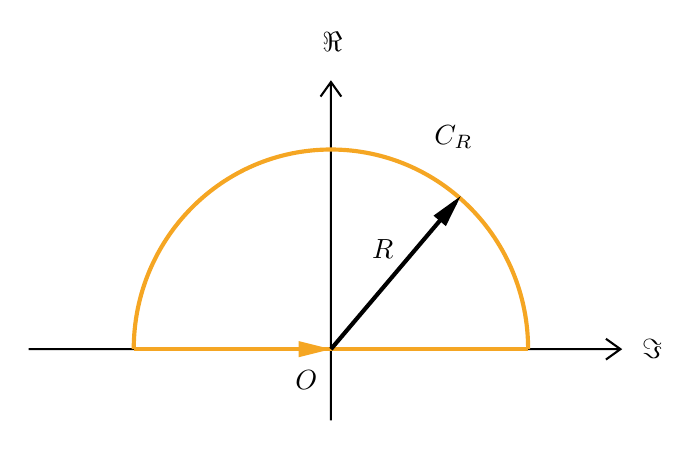
\begin{tikzpicture}[x=0.75pt,y=0.75pt,yscale=-1,xscale=1]
%uncomment if require: \path (0,266); %set diagram left start at 0, and has height of 266

%Shape: Axis 2D [id:dp1282392211894816] 
\draw  (162,181.79) -- (447.09,181.79)(307.61,53.09) -- (307.61,216.09) (440.09,176.79) -- (447.09,181.79) -- (440.09,186.79) (302.61,60.09) -- (307.61,53.09) -- (312.61,60.09)  ;
%Shape: Arc [id:dp1814309272431356] 
\draw  [draw opacity=0][line width=1.5]  (212.6,181.79) .. controls (212.6,181.79) and (212.6,181.79) .. (212.6,181.79) .. controls (212.6,128.66) and (255.14,85.6) .. (307.61,85.6) .. controls (360.08,85.6) and (402.61,128.66) .. (402.61,181.79) -- (307.61,181.79) -- cycle ; \draw  [color={rgb, 255:red, 245; green, 166; blue, 35 }  ,draw opacity=1 ][line width=1.5]  (212.6,181.79) .. controls (212.6,181.79) and (212.6,181.79) .. (212.6,181.79) .. controls (212.6,128.66) and (255.14,85.6) .. (307.61,85.6) .. controls (360.08,85.6) and (402.61,128.66) .. (402.61,181.79) ;  
%Straight Lines [id:da15038694853465828] 
\draw [color={rgb, 255:red, 245; green, 166; blue, 35 }  ,draw opacity=1 ][line width=1.5]    (212.6,181.79) -- (402.61,181.79) ;
\draw [shift={(307.61,181.79)}, rotate = 180] [fill={rgb, 255:red, 245; green, 166; blue, 35 }  ,fill opacity=1 ][line width=0.08]  [draw opacity=0] (15.6,-3.9) -- (0,0) -- (15.6,3.9) -- cycle    ;
%Straight Lines [id:da12449754393780421] 
\draw [color={rgb, 255:red, 0; green, 0; blue, 0 }  ,draw opacity=1 ][line width=1.5]    (307.61,181.79) -- (352.62,128.69) -- (367.5,111.14) ;
\draw [shift={(370.09,108.09)}, rotate = 130.29] [fill={rgb, 255:red, 0; green, 0; blue, 0 }  ,fill opacity=1 ][line width=0.08]  [draw opacity=0] (15.6,-3.9) -- (0,0) -- (15.6,3.9) -- cycle    ;


% Text Node
\draw (289,190.4) node [anchor=north west][inner sep=0.75pt]    {$O$};
% Text Node
\draw (302,27.4) node [anchor=north west][inner sep=0.75pt]    {$\Re $};
% Text Node
\draw (456,175.4) node [anchor=north west][inner sep=0.75pt]    {$\Im $};
% Text Node
\draw (326,127.4) node [anchor=north west][inner sep=0.75pt]    {$R$};
% Text Node
\draw (356,72.4) node [anchor=north west][inner sep=0.75pt]    {$C_{R}$};

% \draw   (239.6, 212.79) circle [x radius= 5, y radius= 5]  (234.6,212.79) -- (244.6,212.79)(239.6,207.79) -- (239.6,217.79) ;
% \draw   (334.61, 116.6) circle [x radius= 5, y radius= 5]  (329.61,116.6) -- (339.61,116.6)(334.61,111.6) -- (334.61,121.6) ;
% \draw   (429.61, 212.79) circle [x radius= 5, y radius= 5]  (424.61,212.79) -- (434.61,212.79)(429.61,207.79) -- (429.61,217.79) ;
% \draw   (396.48, 139.8) circle [x radius= 5, y radius= 5]  (391.48,139.8) -- (401.48,139.8)(396.48,134.8) -- (396.48,144.8) ;
\end{tikzpicture}


\begin{figure}[htb!]
    \centering
    


\tikzset{every picture/.style={line width=0.75pt}} %set default line width to 0.75pt        

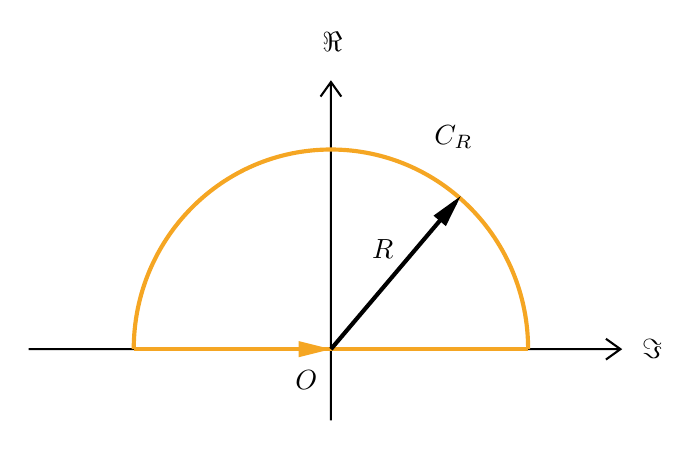
\begin{tikzpicture}[x=0.75pt,y=0.75pt,yscale=-1,xscale=1]
%uncomment if require: \path (0,266); %set diagram left start at 0, and has height of 266

%Shape: Axis 2D [id:dp1282392211894816] 
\draw  (162,181.79) -- (447.09,181.79)(307.61,53.09) -- (307.61,216.09) (440.09,176.79) -- (447.09,181.79) -- (440.09,186.79) (302.61,60.09) -- (307.61,53.09) -- (312.61,60.09)  ;
%Shape: Arc [id:dp1814309272431356] 
\draw  [draw opacity=0][line width=1.5]  (212.6,181.79) .. controls (212.6,181.79) and (212.6,181.79) .. (212.6,181.79) .. controls (212.6,128.66) and (255.14,85.6) .. (307.61,85.6) .. controls (360.08,85.6) and (402.61,128.66) .. (402.61,181.79) -- (307.61,181.79) -- cycle ; \draw  [color={rgb, 255:red, 245; green, 166; blue, 35 }  ,draw opacity=1 ][line width=1.5]  (212.6,181.79) .. controls (212.6,181.79) and (212.6,181.79) .. (212.6,181.79) .. controls (212.6,128.66) and (255.14,85.6) .. (307.61,85.6) .. controls (360.08,85.6) and (402.61,128.66) .. (402.61,181.79) ;  
%Straight Lines [id:da15038694853465828] 
\draw [color={rgb, 255:red, 245; green, 166; blue, 35 }  ,draw opacity=1 ][line width=1.5]    (212.6,181.79) -- (402.61,181.79) ;
\draw [shift={(307.61,181.79)}, rotate = 180] [fill={rgb, 255:red, 245; green, 166; blue, 35 }  ,fill opacity=1 ][line width=0.08]  [draw opacity=0] (15.6,-3.9) -- (0,0) -- (15.6,3.9) -- cycle    ;
%Straight Lines [id:da12449754393780421] 
\draw [color={rgb, 255:red, 0; green, 0; blue, 0 }  ,draw opacity=1 ][line width=1.5]    (307.61,181.79) -- (352.62,128.69) -- (367.5,111.14) ;
\draw [shift={(370.09,108.09)}, rotate = 130.29] [fill={rgb, 255:red, 0; green, 0; blue, 0 }  ,fill opacity=1 ][line width=0.08]  [draw opacity=0] (15.6,-3.9) -- (0,0) -- (15.6,3.9) -- cycle    ;


% Text Node
\draw (289,190.4) node [anchor=north west][inner sep=0.75pt]    {$O$};
% Text Node
\draw (302,27.4) node [anchor=north west][inner sep=0.75pt]    {$\Re $};
% Text Node
\draw (456,175.4) node [anchor=north west][inner sep=0.75pt]    {$\Im $};
% Text Node
\draw (326,127.4) node [anchor=north west][inner sep=0.75pt]    {$R$};
% Text Node
\draw (356,72.4) node [anchor=north west][inner sep=0.75pt]    {$C_{R}$};

% \draw   (239.6, 212.79) circle [x radius= 5, y radius= 5]  (234.6,212.79) -- (244.6,212.79)(239.6,207.79) -- (239.6,217.79) ;
% \draw   (334.61, 116.6) circle [x radius= 5, y radius= 5]  (329.61,116.6) -- (339.61,116.6)(334.61,111.6) -- (334.61,121.6) ;
% \draw   (429.61, 212.79) circle [x radius= 5, y radius= 5]  (424.61,212.79) -- (434.61,212.79)(429.61,207.79) -- (429.61,217.79) ;
% \draw   (396.48, 139.8) circle [x radius= 5, y radius= 5]  (391.48,139.8) -- (401.48,139.8)(396.48,134.8) -- (396.48,144.8) ;
\end{tikzpicture}


    \caption{半圆路径.}
    \label{fig:semicircle}
\end{figure}
下面证明上式第二项为零.一般的对于任意$\theta_1 \leq \theta \leq \theta_2$, 
有$\lim_{R\to \infty} zf(z) = 0$,可以证明对于该角度对应的圆弧$C$有,
\begin{equation}
    \lim_{R \rightarrow \infty} \int_C f(z) dz = 0 .
\end{equation}

\[
    \begin{aligned}
    \lim _{R \rightarrow \infty}\left|\int_C f(z) d z\right| \leq \int_{\theta_1}^{\theta_2} \lim _{R \rightarrow \infty}\left|f\left(R e^{i \theta}\right) i R e^{i \theta}\right| & d \theta \\
    & \leq\left(\theta_2-\theta_1\right) \lim _{R \rightarrow \infty}\left|f\left(R e^{i \theta}\right) R e^{i \theta}\right|=0 .
    \end{aligned}
\]
也就是说,
\begin{equation}
    \int_{-R}^R f(x) d x = 2\pi \imath  \sum_{z_j\in \textrm{上半平面}} \Res f(z_j),
\end{equation}

\begin{example}
    计算\[ 
    I = \int_{-\infty}^{\infty} \frac{dx}{1 + x^2}   .
    \]
\end{example}
\begin{solution}
    由$f(z) = \frac{1}{1+ x^2} = \frac{1}{(z-\imath)(z+\imath)}$可知
    其单极点$\pm \imath$,其中$\imath$在上半平面.
    \[
      \Res f(+\imath) = \frac{1}{2\imath}  
    \]
    因此,$I = 2\pi \imath  \frac{1}{2\imath} = \pi$.由于该积分是一个常见积分
    亦可以通过原函数$\arctan(x)$得到.留数定理的还可以计算这样的积分,
    \[
      I\int_{-\infty}^{\infty} \frac{dx}{(1 + x^2)^n} 
    \]
    具体求解过程参考梁昆淼数学物理方法的解.
\end{solution}


 \subsection{带复指数的定积分}
 考虑以下类型的定积分
 \begin{equation}
    I=\int_{-\infty}^{\infty} f(x) e^{\imath m x} d x
\end{equation}
其中,$m$为正实数;$f(z)$在上半平面除有限个奇点外是解析的,且$\lim_{|z|\to \infty} f(z) = 0, 0 \leq arg z \leq \pi$.
我们使用同样的半圆路径,类似的可以通过留数定理将实轴的积分转换为环路积分求得.
为了使用留数定理,我们先需要证明在半圆上的路径积分为零,这里就要用到\textbf{约旦引理}(Jordan lemma
).
即证明
\begin{equation}
    \lim _{R \rightarrow \infty} \int_{C_R} f(z) e^{\imath m z} d z=0 .
\end{equation}
当$R$足够大时,我们有$|f(z)| < \epsilon$.半圆积分
\begin{align}
    I_R&=\int_0^\pi f\left(R e^{\imath \theta}\right) 
    e^{\imath m R \cos \theta- m R \sin \theta} \imath R e^{\imath \theta} d \theta
    \\
    &\leq \epsilon R \int_0^\pi e^{-m R \sin \theta} d \theta=2 \epsilon R \int_0^{\pi / 2} e^{-m R \sin \theta} d \theta,
\end{align}
可以发现在$\left[ 0, \pi/2\right]$时,
\begin{equation}
    \frac{2}{\pi}\theta \leq \sin{\theta},
\end{equation}
于是有
\begin{equation}
    I_R \leq 2 \epsilon R \int_0^{\pi / 2} e^{-2 m R \theta / \pi} d \theta=2 \epsilon R \frac{1-e^{-m R}}{2 m R / \pi}<\frac{\pi}{m} \epsilon
\end{equation}
即
\begin{equation}
    \lim_{R\to \infty} I_R = 0.
\end{equation}
回到定积分$I$,可以得
\begin{equation}
    \label{eq:complex_exponential_integral}
    I=\int_{-\infty}^{\infty} f(x) e^{ \imath m x} d x = 2\pi \imath \sum_{z_j \in \text{上半平面}} \Res e^{\imath m z_j} f(z_j)
\end{equation}

对于以下类型的积分,可以利用上述结论.如
\begin{equation}
    \int_{0}^{\infty} f(x) \cos {m x} dx, \int_{0}^{\infty} G(x) \sin{m x} dx
\end{equation}
其中,$F(z)$为偶函数,$G(z)$为奇函数,它们在实轴上没有奇点,上半平面上除有限个奇点外解析.
很容易通过$\cos{mx} = \frac{1}{2}\left( e^{\imath m x} + e^{-\imath mx}\right)$等变换得到,即
$$
\begin{aligned}
\int_0^{\infty} F(x) \cos m x d x & =\int_0^{\infty} F(x) \frac{1}{2}\left(e^{\imath m x}+e^{-\imath m x}\right) d x \\
& =\frac{1}{2} \int_0^{\infty} F(x) e^{\imath m x} d x+\frac{1}{2} \int_0^{\infty} F(x) e^{-\imath m x} d x 
\\
& = \frac{1}{2} \int_{-\infty}^{\infty} F(x) e^{\imath m x} d x. 
\end{aligned}
$$

\begin{example}
计算 $\int_0^{\infty} \frac{\cos m x}{x^2+a^2} d x$.
\end{example}
\begin{solution}
偶函数$F(z) e^{\imath m z}=\frac{1}{z^2+a^2} e^{\imath m z}$ 有两个单极点 $\pm a \imath$, 其中 $+a \imath$ 在上半平面. 而 $e^{\imath m z} /\left(z^2+a^2\right)$ 在单极点 $+a \imath$ 的留数为
    $$
    \lim _{z \rightarrow a \imath}\left[(z-a \imath) \frac{e^{\imath m z}}{z^2+a^2}\right]=\lim _{z \rightarrow a \imath}\left[\frac{e^{\imath m z}}{z+a \imath}\right]=\frac{e^{-m a}}{2 a \imath}
    $$
    应用\eqref{eq:complex_exponential_integral},
    $$
    \int_0^{\infty} \frac{\cos m x}{x^2+a^2} d x=\pi \imath \frac{e^{-m a}}{2 a \imath}=\frac{\pi}{2 a} e^{-m a}.
    $$
\end{solution}
\section{Feynman技巧}
我们将讨论下面几个计算定积分的技巧.

\subsection{复变量代换}
以一个例子说明复变量代换的方法.求解定积分
\[
    I =  \int_0^{\infty} e^{-a x} \cos b x d x \\
\]
利用$\cos{bx} = \frac{1}{2}\left( e^{\imath b x} + e^{-\imath bx}\right)$
\[    \begin{aligned}
    I= & \frac{1}{2} \int_{0}^{\infty} \left(e^{-(a-\imath b) x} + e^{-(a + \imath b) x} \right)  d x \\
    = & \frac{1}{2} \left( \frac{1}{a-\imath b} +  \frac{1}{a+\imath b} \right)\\
    = & \frac{a}{a^2+b^2}
\end{aligned}
\]

\subsection{参数微分}
求解定积分
\[
    I =  \int_0^{\infty} x e^{-a x} \cos b x d x \\
\]
我们令
\[
  S(a) =   \int_0^{\infty} e^{-a x} \cos b x d x 
\]
已知 $S(a) = \frac{a}{a^2+b^2}$,通过对$S(a)$对$a$的求导得到
\[
    I = - S'(a)  = \frac{a^2 - b^2}{(a^2 +b^2)^2}    
\]
对于一般的含参数的微分,我们有
\begin{equation}
    \begin{aligned}
    \frac{d}{d \alpha} \int_{x_1(\alpha)}^{x_2(\alpha)} f(x, \alpha) d x= & \int_{x_1}^{x_2} \frac{\partial}{\partial \alpha} f(x, \alpha) d x \\
    & \left[\frac{d x_2(\alpha)}{d \alpha} \right] f(x_2, \alpha)- 
    \left[\frac{d x_1(\alpha)}{d \alpha}\right] f(x_1, \alpha)
    \end{aligned}
\end{equation}

\subsection{被积函数添加函数因子}
求解定积分
\[
    I =  \int_0^{\infty} \frac{\sin{x}}{x} d x 
\]
可以通过乘以一个函数因子$e^{-a x}$来构造参数函数
\[
 S(a) =     \int_0^{\infty}  e^{-a x} \frac{\sin{x}}{x} d x 
\]
这样我们有
\[
  S'(a) = -  \int_0^{\infty}  e^{-a x} \sin{x} d x  = \frac{1}{1+a^2}
\]
对于$a \to \infty$, 有 $S(\infty) = 0$.
而$\frac{1}{1+x^2}$的原函数为$\arctan{x}$,因此
\[S(a) = - \arctan{a} + C\]
可确定$C = \frac{\pi}{2}$,因此我们有$S(a) = \frac{\pi}{2} - \arctan{\alpha}$.
因此,
\[
  I = S(0) = \frac{\pi}{2} .    
\]
该结果我们已通过留数定理求得.
\section{积分求解实例}

\begin{itemize}
    \item 计算定积分 
    $$
    I=\int_0^{\infty} x^{\alpha-1} \frac{1}{1+x} d x \quad(0<\alpha<1).
    $$

    解 将被积函数 $x^{\alpha-1} /(1+x)$ 从实轴延拓到复数 $z$ 平面得到 
    $f(z)=z^{\alpha-1} /(1+z)$. 由于 $f(z)$ 含 有 $z^{\alpha-1}$ ,
    而 $\alpha$ 不是整数,所以 $f(z)$ 是多值函数, 它有两个支点:原点和无限远点. 
    $z$ 每绕原点或 无限远点一圈, 辐角增加 $2 \pi, z^{\alpha-1}$ 多出因子 
    $e^{\imath 2 \pi(\alpha-1)}$ 亦即 $e^{\imath 2 \pi \alpha}$,
     从而 $f(z)$ 也多出这么一个 因子.
    从原点沿着正实轴直至无限远作割线.   
    
    $$
\oint_l f(z) d z=\int_{\epsilon}^R \frac{x^{\alpha-1}}{1+x} d x+\int_{C_R} f(z) d z+\int_R^{\epsilon} \frac{x^{\alpha-1} e^{\imath 2 \pi \alpha}}{1+x} d x+\int_{C_{\epsilon}} f(z) d z .
$$
令 $R \rightarrow \infty, \epsilon \rightarrow 0$.
 上式左边按照留数定理应为 $2 \pi i\{f(z)$ 在有限远各奇点留数之和\}
  右边第一个积分成为所求的 $I$, 第三个积分则成为 $-e^{\imath 2 \pi \alpha} I$. 
  可以证明第 二个和第四个积分则成为零. 事实上,
  $$
\begin{aligned}
\left|\int_{C_R} \frac{z^{\alpha-1}}{1+z} d z\right| & =\left|\int_{C_R} \frac{z^\alpha}{1+z} \frac{d z}{z}\right| \leqslant \max _{\left(C_R \text { 上 }\right)}\left|\frac{z^\alpha}{1+z}\right| \frac{\int|d z|}{|z|} \\
= & \max \frac{R^\alpha}{|1+z|} \cdot \frac{2 \pi R}{R}=2 \pi \max \frac{R^\alpha}{|1+z|} \\
& \sim 2 \pi \frac{1}{R^{1-\alpha} \rightarrow 0} \quad(\text { 于 } R \rightarrow \infty) .
\end{aligned}
$$

$$
\begin{aligned}
\left|\int_{C_{\epsilon}} \frac{z^{\alpha-1}}{1+z} d z\right|= & \left|\int_{C_{\epsilon}} \frac{z^\alpha}{1+z} \frac{d z}{z}\right| \leqslant \max _{\left(C_{\epsilon} \text { 上 }\right)}\left|\frac{z^\alpha}{1+z}\right| \frac{\int|d z|}{|z|} \\
= & \max \frac{\epsilon^\alpha}{|1+z|} \cdot \frac{2 \pi \epsilon}{\epsilon}=2 \pi \max \frac{\epsilon^\alpha}{|1+z|} \\
& \sim 2 \pi \frac{\epsilon^\alpha}{1} \rightarrow 0 \quad(\text { 于 } \epsilon \rightarrow 0) .
\end{aligned}
$$
于是 $\left(1-e^{\imath 2 \pi \alpha}\right) I=2 \pi \imath\{f(z)$ 在有限远各奇点留数之和 $\}$.
$f(z)=z^{\alpha-1}(1+z)^{-1}$ 只有一个单极点 $z_0=-1=e^{\imath \pi}$, 而
$$
\Res f(-1)=\lim _{z \rightarrow-1}[(z+1) f(z)]=\lim _{z \rightarrow-1}\left[z^{\alpha-1}\right]=e^{\imath(\alpha \pi-\pi)}=-e^{\imath \alpha \pi} \text {. }
$$
因此
$$
\begin{aligned}
I & =-\frac{2 \pi \imath e^{\imath \pi \alpha}}{1-e^{\imath 2 \pi \alpha}}=-\frac{2 \pi \imath e^{\imath \pi \alpha}}{e^{\imath \pi \alpha}\left(e^{-\imath \pi \alpha}-e^{\imath \pi \alpha}\right)} \\
& =\frac{2 \pi \imath}{\left(e^{-\imath \pi \alpha}-e^{\imath \pi \alpha}\right)}=\frac{2 \pi \imath}{2 \sin \pi \alpha}=\frac{\pi}{\sin \pi \alpha} .
\end{aligned}
$$

    \item 计算菲涅耳积分(Fresnel integrals)
    $$
    I_1=\int_0^{\infty} \sin \left(x^2\right) \mathrm{d} x \text { 及 } I_2=\int_0^{\infty} \cos \left(x^2\right) \mathrm{d} x \text {. }
    $$

    解 由于 $\sin \left(x^2\right)=\operatorname{Im} e^{\imath x^2}$, 而 $\cos \left(x^2\right)=\operatorname{Re} e^{\imath x^2}$, 所以
$$
I_2+\imath I_1=\int_0^{\infty} e^{\imath x^2} d x .
$$
取图 4-10 所示回路 $l$. 由于 $e^{\mathrm{iz}^2}$ 没有有限远奇点, 所以根据留数定理得
$$
\oint_l e^{\imath z^2} d z=0,
$$
即 $\int_0^R e^{\imath x^2} d x+\int_{C_R} e^{\imath z^2} d z+\int_R^0 e^{\imath\left(\rho e^{\imath \pi / 4}\right)^2} d\left(\rho e^{\imath \pi / 4}\right)=0$,

令 $R \rightarrow \infty$. 第一个积分即所求的 $I_2+\imath I_1$. 第三个积分不难如下算出 :
$$
\begin{aligned}
\lim _{R \rightarrow \infty} \int_R^0 e^{\imath\left(\rho^2 \imath\right)} e^{\imath \pi / 4} d \rho & =\lim _{R \rightarrow \infty}\left(-e^{\imath \pi / 4}\right) \int_0^R e^{-\rho^2} d \rho=-e^{\imath \pi / 4} \int_0^{\infty} e^{-\rho^2} d \rho \\
& =-\frac{\sqrt{\pi}}{2} e^{\imath \pi / 4}=-(1+\imath) \sqrt{\frac{\pi}{8}} .
\end{aligned}
$$
可以证明第二个积分成为零. 为此, 先作一次分部积分,
$$
\int_{C_R} e^{\imath z^2} d z=\left.\frac{e^{\imath z^2}}{2 \imath z}\right|_{z=R} ^{R e^{\imath \pi / 4}}+\int_{C_R} e^{\imath z^2} \frac{\mathrm{d} z}{2 \imath z^2},
$$
其中已积出部分的模
$$
\left|\frac{e^{-R^2}}{2 \imath R e^{\imath \pi / 4}}-\frac{e^{\imath R^2}}{2 \imath R}\right| \leqslant \frac{e^{-R^2}}{2 R}+\frac{1}{2 R} \rightarrow 0 \quad(\text { 于 } R \rightarrow \infty),
$$
未积出部分的模
$$
\begin{aligned}
\left|\int_{C_R} \frac{e^{\imath 2^2}}{2 \imath {z}^2} d z\right| & =\left|\int_{C_R} \frac{e^{-R^2 \sin 2 \varphi+\imath^2 \cos 2 \varphi}}{2 \imath R^2 e^{\imath 2 \varphi}} R e^{\imath \varphi} \imath d \varphi\right| \\
& \leqslant \int_{C_R} \frac{e^{-R^2 \sin 2 \varphi}}{2 R^2} R d \varphi \leqslant \max \left(\frac{e^{-R^2 \sin 2 \varphi}}{2 R}\right) \frac{\pi}{4}
\\
&=\frac{1}{2 R} \frac{\pi}{4} \rightarrow 0 \quad(\text { 于 } R \rightarrow \infty) .
\end{aligned}
$$
于是
$$
\begin{gathered}
I_2+\imath I_1-\sqrt{\frac{\pi}{8}}(1+\imath)=0, \\
I_1=\sqrt{\frac{\pi}{8}}, \quad I_2=\sqrt{\frac{\pi}{8}} .
\end{gathered}
$$
\item 考虑用Feynman技巧来计算
$$
I = \int_0^1 \frac{x^2-1}{\log x} d x
$$
设计这样的函数
$$
G(t):=\int_0^1 \frac{x^t-1}{\log x} d x
$$
$G(0) = 0$,于是问题变为求$G(2)$.不难验证
$$
G^{\prime}(t)=\int_0^1 x^t d x=\frac{1}{t+1}
$$
对$t$求积分后得到
$$
G(2)=\int_0^2 G^{\prime}(t) d t=\int_0^2 \frac{d t}{t+1}=\log 3.
$$

\item 考虑用Feynman技巧来验证高斯积分:
$$
\int_0^{\infty} e^{-x^2} d x = \frac{\sqrt{\pi}}{2}.
$$
\\
定义一个$t$的函数
$$
I(t):=\int_0^{\infty} \frac{e^{-x^2}}{1+(x / t)^2} d x, t>0. 
$$
于是菲涅尔积分就是求$I_1 = I(\infty)$.
做代换$x/t=y$后,并换回积分变量为$x$有 $$
I(t)=t \int_0^{\infty} \frac{e^{-t^2 x^2}}{1+x^2} d x
$$
可以得到 $$
\lim _{t \rightarrow 0} \frac{I(t)}{t}=\frac{\pi}{2}.
$$
为了能利用上面的技巧,我们将考虑
$$
e^{-t^2} I(t)=t \int_0^{\infty} \frac{e^{-t^2\left(1+x^2\right)}}{1+x^2} d x
$$
对于
$$
\frac{d}{d t}\left(t^{-1} e^{-t^2} I(t)\right)=\int_0^{\infty}-2 t e^{-t^2\left(1+x^2\right)} d x=-2 e^{-t^2} \int_0^{\infty} e^{-u^2} d u=-2 e^{-t^2} I(\infty)
$$

两边积分
$$
\underbrace{\int_0^{\infty} \frac{d}{d t}\left(t^{-1} e^{-t^2} I(t)\right) d t}_{=-\lim _{t \rightarrow 0} \frac{I(t)}{t}}=\underbrace{\int_0^{\infty}-2 e^{-t^2} I(\infty) d t}_{=-2 I(\infty)^2}
$$
得到
$$
I(\infty) = \sqrt{\frac{\pi}{4}} = \frac{\sqrt{\pi}}{2}.
$$

\end{itemize}
% \input{infinite_range.tex}
    \caption{复变函数积分示意图.光滑曲线$\ell$上取一系列点$z_k$将其分成$n$小段.}
    \label{fig:complex_integral}
\end{figure}
当$n\to \infty$, 求和则转化为积分.当这个和的极限存在且
与$\xi_k$的选取无关时,这个极限称为
函数$f(z)$沿着路径$\ell$的\textbf{路径积分}(Contour integral), 记作
$\int_{\ell} f(z) dz$,即
\begin{equation}
    \int_{\ell} f(z) dz = \lim_{n\to \infty} \sum_{i=k}^{n} f(\xi_k) (z_{k} - z_{k-1}) . 
\end{equation}
其实,我们还可以将该定义用实虚部的方式表达出来,
\begin{align}
    \int_{\ell} f(z) dz  & = \int_{\ell} \left( u(x,y) + \imath v(x,y) \right) (dx + \imath dy) 
    \\
    & = \int_{\ell} \left( u(x,y) dx  -  v(x,y) dy \right) + \imath \int_{\ell}  \left( v(x,y) dx  + u(x,y)dy \right) 
\end{align}
这样一来,复变函数的路径积分就转化成了两个实变函数的线积分.因此,很多实函数线积分的性质可以应用在路径积分上.


